\chapter{Východisková kapitola}

\label{kap:vychodiska} % id kapitoly pre prikaz ref


\section{Sémantický web} \label{secSemanticWeb}
Sémantický web, podľa \cite{scientificAmerican} je rozšírením súčasného webu. Väčšina obsahu, ktorý sa v
súčasnosti na webe nachádza je navrhnutá pre ľudí. Programy dokážu rozpoznať, aká
časť stránky je hlavička, kde sa nachádza odkaz na inú stránku, avšak nedokážu pochopiť význam
toho, čo sa vlastne v jednotlivých častiach nachádza. Riešením má byť práve sémantický web, ktorý umožňuje reprezentovať a voľne publikovať dáta v nejakom vhodnom jazyku (RDF, viď. \ref{secRdf}), ktorý im umožňuje priradiť aj význam. Tradičné systémy na reprezentáciu poznatkov boli väčšinou centralizované, čo si vyžadovalo jednotné definície bežných pojmov. Takáto centrálna kontrola sa však kvôli
neustálemu rozrastaniu systému stáva nezvládnuteľnou, a teda definície a významy priradzujeme použitím ontológií (viď. \ref{secOntology}).

Semantic Web Stack, prípadne Semantic Web (Layer) Cake ilustruje štruktúru sémantického webu. Na obr. \ref{semanticLayerCake} vidíme ako sú organizované technológie, ktoré sú pre tento web
štandardizované. Každá vrstva využíva schopnosti nižšej vrstvy. Tieto vrstvy môžeme rozdeliť do 3 skupín a na základe \cite{semanticWebLayer2} ich definovať nasledovne:

\begin{itemize}
\item Pojmy zo spodnej vrstvy poznáme už z hypertextového webu. Z toho vyplýva, že sémantický web je iba rozšírením klasického webu. URI (viď. \ref{secUri}) umožňujú jednoznačne identifikovať zdroje. UNICODE je kódovanie slúžiace na reprezentáciu a spracovanie textov v rôznych jazykoch. XML, XML Query, XML Schema a XML Namespaces boli vyvinuté a štandardizované konzorciom W3C. XML je značkovací jazyk, ktorý umožňuje vytvárať dokumenty so štruktúrovanými dátami, ktorým sémantický web dodáva význam.
XML Query je štandardizovaný jazyk na kombinovanie dokumentov, databáz, či webových stránok, umožňuje robiť dopyty nad XML dátami. XML Schema je jazyk na vyjadrenie obmedzení o XML dokumentoch a špecifikuje, ako formálne opísať prvky v týchto dokumentoch. Názvy elementov si definuje autor XML dokumentu. Pri spájaní viacerých dokumentov môže dochádzať ku konfliktu názvov v prípade, keď je rovnaký názov použitý s iným významom. Práve tento problém riešia XML Namespaces. Vytvorením prefixu pre namespace a následným používaním prefixu využívame názvy elementov v takom kontexte, v akom sú definované v nami vybranom namespace. 

\item Druhou skupinou, nachádzajúcou sa v strede, sú technológie štandardizované W3C. Umožňujú budovať aplikácie sémantického webu. Sú nimi RDF Model a Syntax (viď. \ref{secRdf}), RDF Schema (viď. \ref{secSchema}) a Ontológie (viď. \ref{secOntology}). RDF je dátový model, v ktorom vyjadrujeme vzťah medzi hocijakými dvoma zdrojmi vo forme trojice (subjekt, predikát, objekt). RDF Schema (RDFS) je univerzálny jazyk, ktorý umožňuje definovať nové slovníky. Ontológie, v užšom ponímaní slovníky, sú súbory pojmov a vzťahov medzi pojmami z určitej časti sveta, ktorá nás zaujíma.

\item Treťou skupinou sú technológie, ktoré štandardizované zatiaľ nie sú alebo sú iba nápadmi. Na základe súborov pravidiel vieme pomocou logiky odvádzať nové informácie. Tieto odvodené informácie podporujeme dôkazmi. Najvyššie sa nachádza trust(pravda), teda mechanizmus, ktorým by sme vedeli určiť, ktorým informáciám môžeme dôverovať. 
\end{itemize}

\begin{figure}[h]
\centering
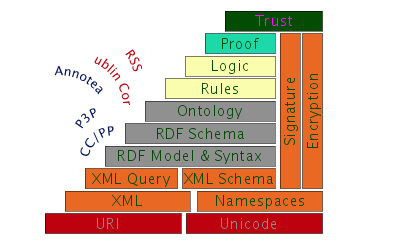
\includegraphics[width=0.6\textwidth]{images/semanticLayerCake}
\caption{Semantic Web Layer Cake, zdroj: \cite{semanticWebLayer}}
\label{semanticLayerCake}
\end{figure}

\subsection{Linked Open Data} \label{secLinkedData}
Termín Linked Data, spracovaný podľa \cite{linkedData}, označuje súbor všetkých dát publikovaných na webe pomocou technológií sémantického webu. Ide v postate o sémantický web aplikovaný do praxe. Ak sú linked data, teda prepojené údaje, voľne dostupné na opätovné použitie označujeme ich termínom Linked Open Data. Linked Open Data sú silnou kombináciou prepojených a otvorených údajov. Jedným z pozoruhodných príkladov LOD je je DBpedia –
snaha o získanie štruktúrovaných informácií z Wikipedie a ich sprístupnenie na webe.

Zásady pri tvorbe prepojených údajov (Linked data principles)predstavil Tim Berners-Lee. Ide o tieto pravidlá:

\begin{enumerate}
\item Používajte URI ako názvy objektov.
\item Používajte identifikátory URI protokolu HTTP, aby ľudia mohli tieto mená vyhľadať.
\item Keď niekto vyhľadá URI, poskytnite užitočné informácie o tom, čo názov identifikuje pomocou otvorených štandardov, ako sú napr. RDF alebo SPARQL.
\item Zahrňte odkazy na ďalšie URIs, aby ľudia mohli dohľadať ďalšie informácie.
\end{enumerate}

Štvrtý princíp prepojených údajov podporuje použitie hypertextových odkazov nie
len medzi webovými dokumentami, ale medzi ľubovoľnými objektami, napr. odkaz
medzi človekom a miestom, alebo medzi miestom a spoločnosťou. Oproti klasickému
webu však majú tieto odkazy aj typy, teda napr. medzi dvoma ľuďmi môže mať odkaz
typ priateľ.

Podľa \cite{linkedData5star}, Tim Berners-Lee navrhol 5-hviezdičkovú schému rozvinutia linked open data.

\begin{itemize}
\item Jednu hviezdičku získajú dáta, ktoré sú sprístupnené na webe v ľubovoľnom formáte pod otvorenou licenciou. Môžeme si ich prečítať, zdieľať, meniť, je jednoduché ich poskytnúť, avšak dáta sú uzavrené vrámci dokumentu a je ťažké ich z neho dostať.
\item Dve hviezdičky získajú dáta, ktoré sú sprístupnené v štruktúrovanej podobe, je možné ich spracovať a proprietárnym softvérom získať agregácie, či výpočty. Dáta sú však stále uzavreté vrámci dokumentu a ich získanie závisí od proprietárneho softvéru.
\item Tri hviezdičky sú priradené dátam, ktoré sú sprístupnené v neproprietárnom otvorenom formáte.
\item Štyroma hviezdičkami sú hodnotené dáta, v ktorých používame URI na určenie vecí tak, aby sa na nich mohli ľudia odkazovať. Takéto dáta je bezpečné kombinovať s inými dátami, keďže vieme, že v prípade rovnakého URI ide o rovnakú vec. Najbežnejším spôsobom reprezentácie dát je použitie RDF.
\item Päť hviezdičiek, a teda najlepšie hodnotenie, získavajú dáta, ktoré sú nalinkované na iné. Vytvárame tým kontext a umožňuje nám to objavovať ďalšie súvisiace dáta.
\end{itemize}

\subsection{RDF} \label{secRdf}
Táto podkapitola je spracovaná podľa \cite{rdf, rdf2}. RDF je skratka pre Resource Description
Framework. Doteraz je to najjednoduchší a zároveň najsilnejší z formátov, ktorý poskytuje spôsob na vyjadrovanie informácií o zdrojoch. Zdrojom môže byť hocičo, teda dokument, osoba, fyzický objekt a podobne. RDF bol vyvinutý a odsúhlasený W3C. Je určený pre situácie, pri ktorých informácie na
webe musia byť spracovávané prevažne aplikáciami, nie len zobrazované ľuďom.

RDF dáta sú zložené z tvrdení. Tvrdenie, v RDF nazývané aj trojica,resp. triple, umožňuje vyjadriť vzťah medzi dvoma zdrojmi a má vždy nasledujúcu štruktúru:

\begin{center}
<subjekt> <predikát> <objekt>
\end{center}
Príklad trojice, vyjadrujúci informáciu, že Mount Everest je najvyšší vrch v Himalájach:
\begin{center}
<Himaláje> <najvyšší vrch> <Mount Everest>
\end{center}

Pre lepšie pochopenie môžeme RDF dáta skúsiť porovnať s dátami v relačnej databáze, kde sú údaje uložené v tabuľkách. Zisťujeme, že v podstate bunka v tabuľke je prezentovaná tiež troma hodnotami. Identifikátor pre riadok sa nazýva subjekt, je to vec, o ktorej daný výrok hovorí. Identifikátor pre stĺpec sa
nazýva predikát, hovorí o nejakej vlastnosti entity daného riadka(subjektu) a hodnota
v bunke sa nazýva objekt. Ak by sme teda chceli dáta z relačnej databázy pretransformovať na dáta v RDF formáte, dalo by sa to pomerne jednoducho. V prípade opačného smeru, teda zmeny ľubovoľných RDF dát na relačnú databázu by bolo problémom, že predikáty nie sú pevne dané, a teda jediné, čo by sme vedeli s istotou vytvoriť by bola jedna veľká tabuľka s 3 stĺpcami, pričom každý riadok by vyjadroval jeden triple.

Trojice sa stávajú zaujímavejšími, keď viac ako jedna trojica opisuje rovnakú entitu, teda zdroj.
V tom prípade je výhodné vizualizovať ich pomocou súvislého orientovaného grafu, pričom subjekt a objekt sú vrcholmi grafu a predikát je hrana medzi nimi. Skupina rovnakých tvrdení, môže byť preložená do rôznych syntaxí, avšak vždy budú predstavovať ten istý graf. Medzi formáty pre písanie RDF grafov patria Turtle family
of RDF languages (N-Triples, Turtle, TriG, N-Quads), JSON-LD, RDFa, RDF/XML. 
Vyššie uvedená trojica (<Himaláje> <najvyšší vrch> <Mount Everest>) vyjadrená použitím Turtle syntaxe:   
\begin{center}
dbr:Himalayas dbp:highest dbr:Mount\_Everest
\end{center}

RDF je teda predovšetkým systém na modelovanie údajov. Každý vzťah medzi
hocijakými dvoma entitami je presne reprezentovaný, čo umožňuje veľmi
jednoduché spájanie údajov z viacerých zdrojov. Dôvodom ľahkého spájania je to, že nie je potrebné usporiadávať
stĺpce tabuliek, obávať sa chýbajúcich údajov konkrétneho stĺpca a podobne, keďže
vzťah buď existuje alebo nie.

Jednotlivé časti trojice (subjekt, predikát a objekt) môžu byť rôzne reprezentované. 
Prostredníctvom IRIs (viď. \ref{secUri}) môžeme vyjadriť subjekt, objekt aj predikát. Literály, jednoduché hodnoty ako sú reťazce, dátumy, čísla, môžu vystupovať iba ako objekt. V pozícií objektu a subjektu môžu vystupovať aj tzv. blank nodes. Sú to prázdne uzly, ktoré sa môžu použiť na označenie zdrojov bez toho, aby boli výslovne pomenované. Naznačujú teda existenciu nejakej veci, ktorá však nie je definovaná prostredníctvom IRI. 

Príklad blank node (\_:someone):
\begin{verbatim}
@prefix xsd: <http://www.w3.org/2001/XMLSchema#>.
@prefix foaf: <http://xmlns.com/foaf/0.1/>
@prefix ex: <http://example.org/example#>.

ex:Jane foaf:knows _:someone.
_:someone foaf:name "John"^^xsd:string.
\end{verbatim}

Na obr. \ref{orientovanyGraf} vidíme graf vyjadrujúci informácie o Mount Evereste, Himalájach a Jozefovi Psotkovi. Tento graf vznikol použítím Turtle syntaxe. Tá je najčitateľnejšia pre ľudí.

\begin{figure}[h]
\centering
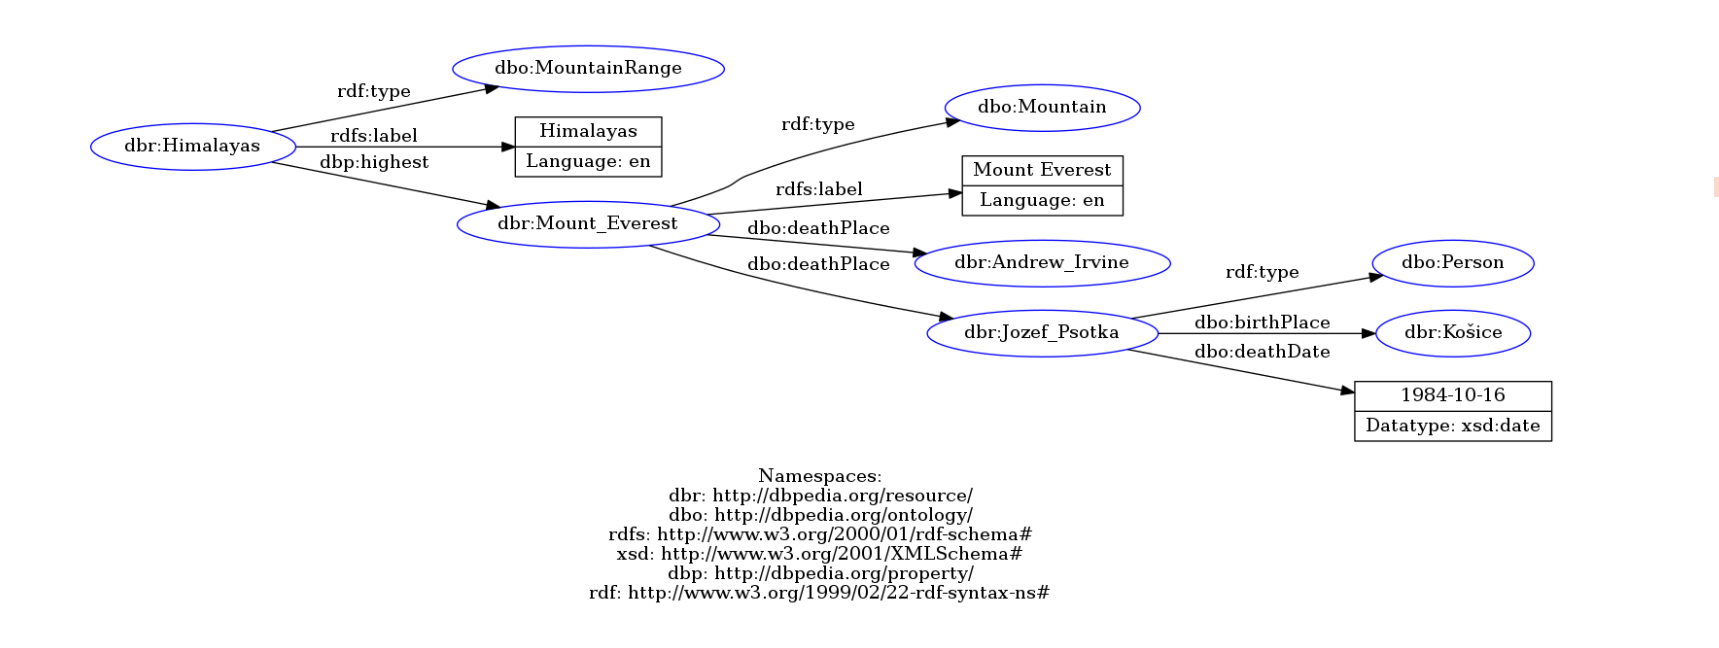
\includegraphics[width=\textwidth]{images/orientovanyGraf}
\caption{Orientovaný graf, ktorý vznikol na základe nižšie uvedeného kódu}
\label{orientovanyGraf}
\end{figure}

\begin{verbatim}
@prefix dbr: <http://dbpedia.org/resource/>.
@prefix dbo: <http://dbpedia.org/ontology/>.
@prefix rdfs: <http://www.w3.org/2000/01/rdf-schema#>.
@prefix xsd: <http://www.w3.org/2001/XMLSchema#>.
@prefix dbp: <http://dbpedia.org/property/>.
@prefix rdf: <http://www.w3.org/1999/02/22-rdf-syntax-ns#>.
dbr:Himalayas
a dbo:MountainRange;
rdfs:label "Himalayas"@en;
dbp:highest dbr:Mount_Everest.

dbr:Mount_Everest
a dbo:Mountain;
rdfs:label "Mount Everest"@en;
dbo:deathPlace dbr:Andrew_Irvine;
dbo:deathPlace dbr:Jozef_Psotka.

dbr:Jozef_Psotka
a dbo:Person;
dbo:birthPlace dbr:Košice;
dbo:deathDate "1984-10-16"^^xsd:date.
\end{verbatim}

\subsection{URI} \label{secUri}
URI, podľa \cite{rdf2} ponúka globálnu identifikáciu pre zdroje na celom webe. Jeho syntax
umožňuje „dereferenciu“ - použitie všetkých informácií v URI (ktoré špecifikujú meno
servera, protokol, číslo portu, meno súboru a podobne) na to, aby lokalizovali súbor.
Ak všetky časti fungujú, vtedy môžeme vyhlásiť, že URI je zároveň aj URL, teda
URL je špeciálnym prípadom URI. Avšak tento rozdiel nie je podstatný z pohľadu
modelovania. Vieme, že ak ukazujú dva vrcholy v RDF grafe na rovnaké URI, ide o ten
istý vrchol. Na základe \cite{rdf} vieme, že IRI je skratka pre International Resource Identifier,
a je zovšeobecnením URI. V reťazci IRI môžu byť použité aj znaky, ktoré nie sú v ASCII.

\subsection{Ontológie a slovníky} \label{secOntology}
\subsubsection{Ontológie}
Ontológia \cite{owl} je súborom presných tvrdení o nejakej časti sveta, ktorá nás zaujíma. Zvyčajne máme k dispozícií množiny pojmov a vzťahy medzi nimi. Označujeme ich ako doménu záujmu alebo predmet ontológie. Jednotlivé tvrdenia sú prezentované ako
triedy a vzťahy, a vytvárajú hierarchickú štruktúru celej ontológie.
Súčasťou ontológií sú takisto aj obmedzenia a pravidlá, pomocou ktorých je
možné odvádzať nové fakty, ktoré neboli explicitne uvedené. Presnými
opismi v ontológiách predchádzame nedorozumeniam, ku ktorým môže dochádzať v
oblasti ľudskej komunikácie a zabezpečujeme, aby sa softvér správal jednotne a predvídateľne.

\subsubsection{Slovníky(vocabularies)}
Podľa \cite{rdf, vocabularies}, jednotlivé vyhlásenia, ktoré o zdrojoch robíme síce obsahujú IRIs, avšak
dátový model nemá žiadne vedomosti o tom, čo v skutočnosti znamenajú. V praxi sa
teda využívajú slovníky, ktoré na sémantickom webe definujú pojmy a vzťahy používané na opis a reprezentáciu nejakej oblasti záujmu. Tú následne využívame v nejakej
konkrétnej aplikácií. Slovník je základným stavebným kameňom inferenčných techník
na sémantickom webe. Príklady existujúcich slovníkov:
\begin{itemize}
\item FOAF, teda „Friend of a Friend“, je jedným z prvých RDF slovníkov používaných na celom svete. Popisuje ľudí, ich aktivity a interakciu s inými ľuďmi. Umožňuje rôznym skupinám ľudí popísať napr. sociálne siete bez potreby centralizovanej databázy. 
\item SKOS, teda Simple Knowledge Organization System, a je využívaný najmä ľuďmi zaoberajúcimi sa informatikou a knihovníkmi.
\item DC:Dublin Core, skupina termínov, ktoré sa používajú na opis digitálnych zdrojov (obrázky, webové stránky,...) alebo fyzických zdrojov (knihy, umelecké diela,...). Zahŕňajú vlastnosti ako napríklad "creator", "publisher" alebo "title". 
\item RDF Schema, popísaná v podkapitole \ref{secSchema}
\end{itemize}


\subsubsection{Porovnanie slovníkov a ontológií}
Úlohou ontológií a slovníkov je teda pomáhať pri spájaní dát na sémantickom webe. Predchádzame tým napríklad prípadu, že
v dvoch rôznych dátových množinách by boli použité rovnaké pojmy s rôznym významom. 

Čo sa týka rozdielu medzi ontológiami a slovníkmi, podľa \cite{vocabularies}, neexistuje presný
rozdiel, na základe ktorého by sme mohli tvrdiť, že niečo je určite slovník a niečo je určite
ontológia. Pojmom ontológia označujeme komplexnejšiu množinu dát, a teda za hlavný
rozdiel by sa dala považovať úroveň abstrakcie a vzťahov vrámci obsahu. Pri tvorbe
ontológií sa využívajú existujúce slovníky na zníženie úsilia, ktoré musíme vynaložiť na
budovanie ontológie od nuly.

\subsection{RDF Schema} \label{secSchema}
RDF Schema \cite{schema} je slovníkom pre modelovanie RDF dát. Poskytuje spôsob na opísanie skupín zdrojov, ktoré spolu súvisia a vzťahov medzi týmito zdrojmi. 
Triedy a vlastnosti v RDFS by mohli byť paralelou k triedam a atribútom používaným v objektovo-orientovaných
programovacích jazykoch. 

Príkladom tried z RDFS je rdfs:Resource, čo je trieda, do ktorej patrí každý zdroj. Ďalej trieda rdfs:Literal, vyjadrujúca hodnoty ako čísla, či textové reťazce alebo rdfs:Container, čo je trieda RDF kontainerov, ktoré by sme mohli prirovnať k akýmsi poliam alebo množinám v programovacích jazykoch.

Príkladom vlastností z RDFS sú  rdfs:subClassOf, teda vlastnosť byť podtriedou, rdfs:domain, vlastnosť vyjadrujúca doménu nejakého vzťahu,
rdfs:comment, popis subjektu alebo rdfs:seeAlso, teda nejaké ďalšie informácie o subjekte.

\subsection{OWL} \label{secOwl}
Na základe \cite{owl} je OWL deklaratívny jazyk, teda logickým spôsobom popisuje stav vecí.
Využíva sa na vyjadrenie ontológií a v podstate je rozšírením RDFS (viď. \ref{secSchema}), napr. o termy,
ktoré popisujú množinové operácie. Pomocou nástrojov na odvodzovanie je možné prinášať nové informácie a vytvárať závery, ktoré vyplývajú z toho, čo sme zadefinovali.
Spôsob, akým sa tieto závery odvodzujú však závisí od konkrétnych implementácií a nie
je súčasťou OWL dokumentu. Existujú rôzne syntaxe pre OWL, ktoré slúžia na rôzne
účely, napr. RDF/XML syntax, ktorá ako jediná musí byť podporovaná všetkými nástrojmi OWL. Príklady rôznej syntaxe vidíme nižšie a je v nich vyjadrená hierarchia
medzi triedami Dog a Pet, teda vlastnosť byť podtriedou. 

\begin{verbatim}
Functional-Style Syntax
SubClassOf(:Dog :Pet)

RDF/XML Syntax
<owl:Class rdf:about="Dog">
<rdfs:subClassOf rdf:resource="Pet"/>
</owl:Class>

Turtle Syntax
:Dog rdfs:subClassOf :Pet .

Manchester Syntax
Class: Dog
SubClassOf: Pet

OWL/XML Syntax
<SubClassOf>
<Class IRI="Dog"/>
<Class IRI="Pet"/>
</SubClassOf>
\end{verbatim}

\subsection{SPARQL} \label{secSparql}
SPARQL, spracovaný na základe zdrojov \cite{sparql, sparql2}, je jazyk navrhnutý na vytváranie
dopytov nad RDF dátami. Kľúčovými slovami v dopytoch sú PREFIX, SELECT,
WHERE. Využívať môžeme aj FROM, ORDER BY, LIMIT a podobné výrazy,
ktoré sú využívané aj v SQL dopytoch. Podmienky vo WHERE časti píšeme vo forme
trojíc, ktoré sú podobné trojiciam v RDF, ale môžu obsahovať premenné. Tie zvyšujú flexibilitu pri porovnávaní s RDF dátami. Takisto sú podporované aj
ASK dopyty, ktoré vracajú boolean hodnoty a CONSTRUCT dopyty,
pomocou ktorých môžeme vytvárať RDF grafy z výsledkov dopytov.

Ak chceme robiť dopyty nad dátami nepotrebujeme žiaden špeciálny softvér, keďže
kolekcie dát sú často dostupné prostredníctvom SPARQL endpointov. Je to webová
služba, ktorá akceptuje SPARQL dopyty a vracia výsledky. DBpedia je najpopulárnejším SPARQL endpointom.

Nižšie môžeme vidieť dopyt nad endpointom DBpedia
 (\href{http://dbpedia.org/snorql/}{http://dbpedia.org/snorql/}).
Na základe neho dostávame zoznam vrchov, obr. \ref{dopyt}, ktoré patria do triedy dbo:Mountain a zároveň sa nachádzajú v pohorí Himaláje.
Prefix rdf:type, teda príslušnosť k určitej triede, sme nahradili skratkou a. Vo výslednom zozname je každý vrch popísaný prislúchajúcim URI, takže sa prostredníctvom neho môžeme dostať
k ďalším informáciám o vybranom vrchu.

\begin{verbatim}
PREFIX dbo: <http://dbpedia.org/ontology/>
SELECT ?peak WHERE {
?peak a dbo:Mountain;
dbo:mountainRange :Himalayas.
}
\end{verbatim}

\begin{figure}[h]
\centering
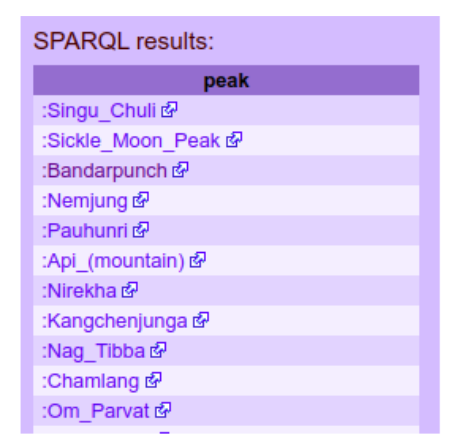
\includegraphics[width=0.3\textwidth]{images/dopytDBpedia}
\caption{Výsledok dopytu nad DBpedia}
\label{dopyt}
\end{figure}

\subsection{Triplestore} \label{secTriplestore}
RDF Triplestore je podľa \cite{triplestore} typ grafovej databázy, v ktorej sú uložené sémantické
fakty. Triplestory sú uprednostňované na manažovanie prepojených dát, sú fexibilnejšie
a lacnejšie ako relačná databáza. Zvládajú sémantické dopyty a používanie odvodzovania na zistenie nových informácií z už existujúcich vzťahov.


\section{Existujúce riešenia} 
Táto kapitola sa venuje už existujúcim riešeniam daného problému. Uvádzam bakalársku prácu, ktorá sa touto témou zaoberala minulý rok a vybrala som si jednu slovenskú
a jednu zahraničnú webovú aplikáciu, na ktorých je k dispozícií veľké množstvo receptov nie len ako jeden blok textu, ale ako dáta, s ktorými je možné pracovať.

\subsection{Varecha}

\begin{figure}[h]
\centering
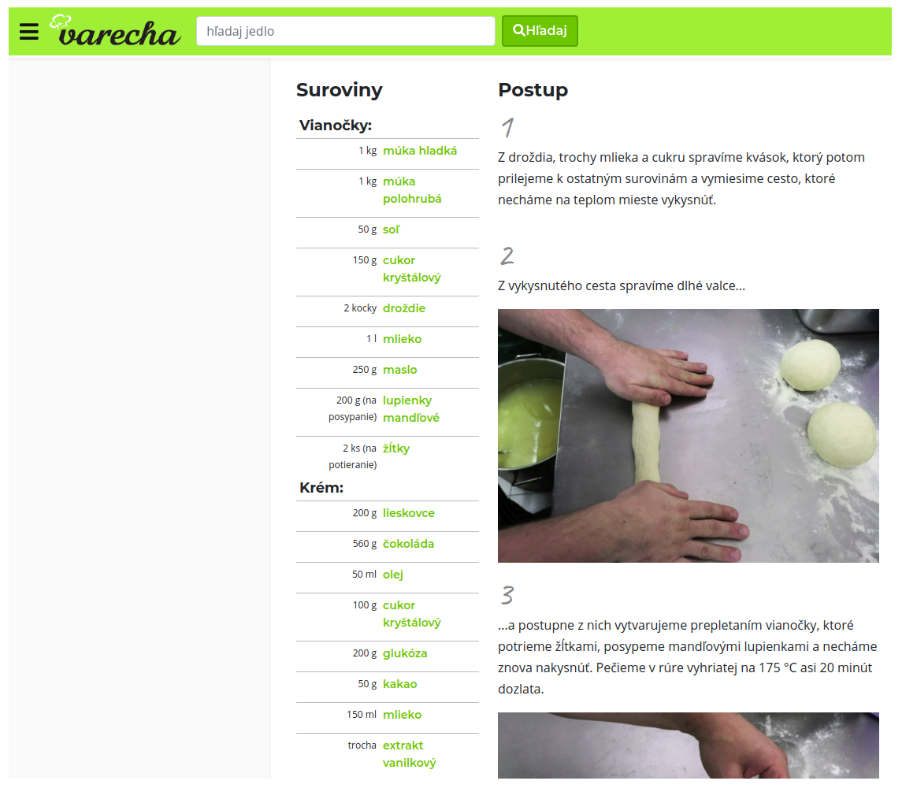
\includegraphics[width=0.7\textwidth]{images/varecha}
\caption{Recept na vianočku, zdroj: \cite{varecha}}
\label{varecha}
\end{figure}

Tento slovenský internetový portál \cite{varecha} vznikol v roku 2009, pričom stihol zverejniť viac
než 60 tisíc receptov. Pre neprihlásených používateľov je možnosť vyhľadávať recepty
podľa druhov jedál, krajín, ingrediencií, atď. Pre prihlásených je dostupné aj vytváranie
vlastného receptu, pridávanie komentárov, vlastných poznámok.

Vytváranie vlastného receptu, je zaujímavejšie, keďže nám vlastne predstavuje jeho
jednotlivé časti. Samostatne sú vypĺňané informácie ako názov, úvodný popis, čas varenia, či tepelnej úpravy, množstvo porcií a podobne. Zaradzovanie do rôznych kategórií
funguje na základe toho, že autor sám usúdi, kam sa recept hodí a danú kategóriu
zaklikne. V prípade surovín je možnosť rozdeľovať ich na základe toho, v ktorej časti
jedla sa využijú, pridávať ich množstvá a jednotky. Pri udaní názvu ingrediencie, ktorý
web dokáže rozpoznať, je možné sa dostať kliknutím na ňu k jej nutričným hodnotám
alebo ďalším jedlám, v ktorých sa využíva. Samotný postup je odkrokovaný, avšak nikde nie je presnejšie povedané, ako by mal daný krok vyzerať, a teda je to na úvážení
autora, čo tam uvedie. Ukážku receptu so surovinami a postupom vidíme na obr. \ref{varecha}.

\subsection{Yummly}

\begin{figure}[h]
\centering
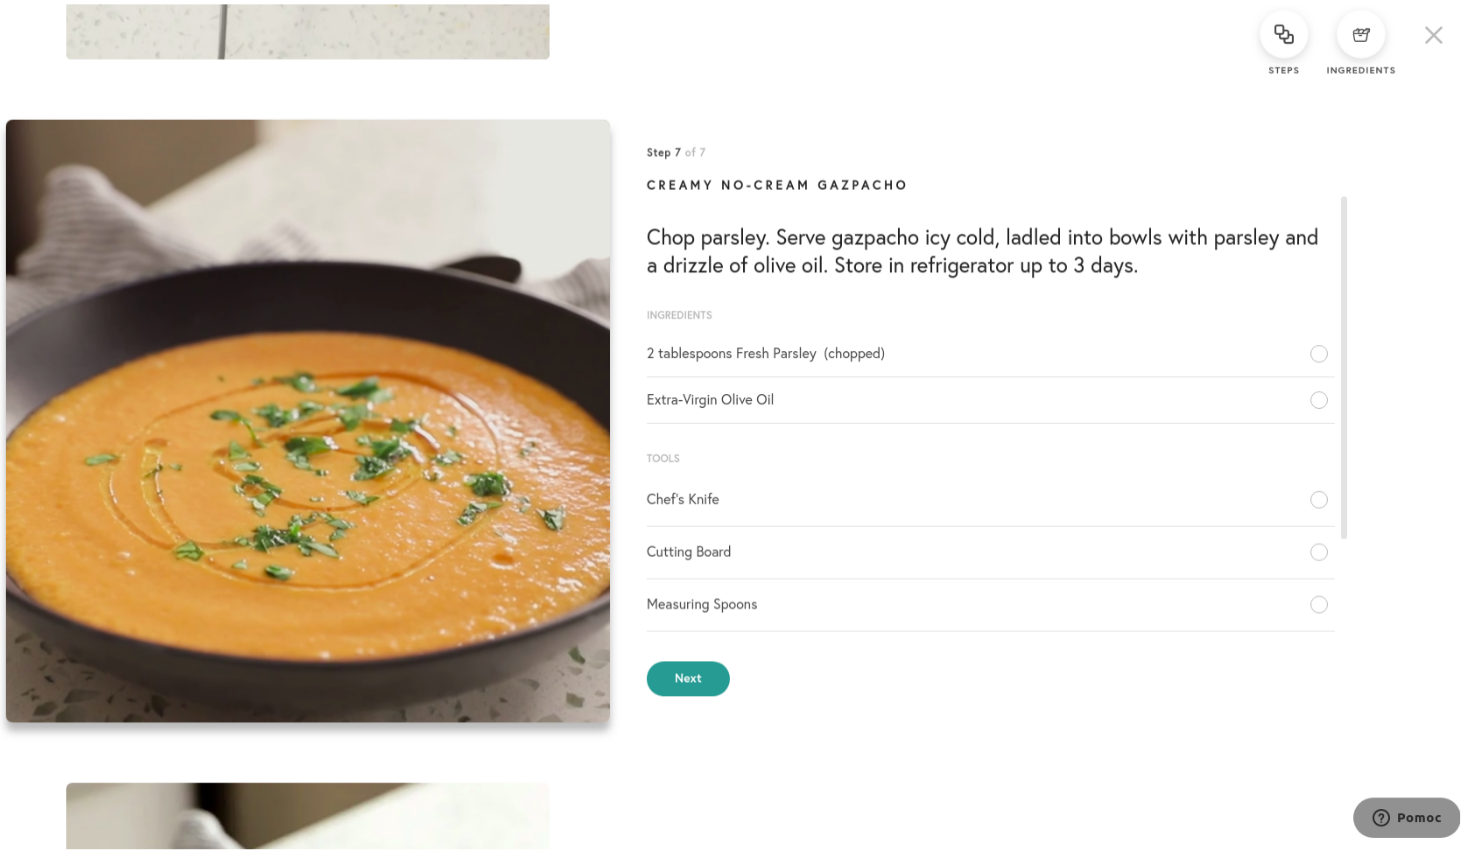
\includegraphics[width=0.8\textwidth]{images/yummly}
\caption{Recept na gazpacho, zdroj: \cite{yummly}}
\label{yummly}
\end{figure}

Podľa informácií na stránke \cite{yummly} je tu k dispozícií viac ako 2 milióny receptov a má
približne 26 miliónov používateľov. V prípade, že sme prihlásení, môžeme si v profile
nastavovať rôzne preferencie, diéty, alergie a chute. Na základe všetkých týchto informácií nám aplikácia dokáže poskytovať stále relevantnejšie údaje bez toho, aby sme to
museli vždy sami vyhľadávať.

Niektoré ingrediencie sa dajú jedným kliknutím na nich dohľadať priamo v obchode.
Čo sa týka vyhľadávania, okrem bežných parametrov, ktoré sme si uviedli napr. aj pri
portály Varecha \cite{varecha}, je možné vyhľadávať jedlá na základe spôsobu prípravy. Popisy
postupov boli takisto podobné, pri videorecepte však boli aj samostatne uvedené nádoby, či iné zariadenia a zároveň aj ingrediencie potrebné na vykonanie daného kroku,
tak ako vidíme na obr. \ref{yummly}. Nachádzajú sa tu však aj recepty, ktoré ako postup
obsahovali odkaz na článok alebo inú stránku.


\subsection{Bakalárska práca Inteligentný receptár na báze prepojených dát}
Téme vytvárania receptov sa venovala minuloročná bakalárska práca \cite{bakalarka}. Jej cieľom
bolo najmä navrhnúť a implementovať webovú aplikáciu, ktorá spravuje a zobrazuje
dáta nad štandardom sémantického webu.

Došlo k preskúmaniu existujúcich LOD zdrojov venujúcich sa tejto tématike, a
zároveň k návrhu vlastnej ontológie. Jej hlavnou triedou bola trieda Recipe, ktorá popisovala samotný recept. Ten má dva hlavné atribúty, ktoré tvoria každý recept. Sú
nimi ingrediencie a postup. Zoznam ingrediencií, a následne samotná ingrediencia sú
reprezentované samostatnými triedami. Každá ingrediencia má nejakú jednotku merania a zároveň množstvo. Tieto vlastnosti sú popísané triedou Mass. Postup je v tejto
ontológií reprezentovaný ako pole reťazcov. Ďalšími atribútmi prislúchajúcimi k triede
Recipe sú autor, čas prípravy, počet porcií, kategórie, a zároveň hodnotenie, ktoré má
tiež samostatnú triedu.

Začiatočné dáta boli čerpané zo stránky DBpedia. Na ich uskladnenie bol využitý
triple store TDB, ktorý je komponentom Jeny, čo je voľne dostupný Java framework
pre vytváranie sémantického webu. Dopyty a aktualizácie boli vykonávané na SPARQL
server Fuseki. Ten je spojený s TDB, používaného na trvalé uskladnenie dát. Pri pripojení na server a následné dopytovanie a aktualizáciu dát bola využitá knižnica EasyRdf,
ktorá nám umožňuje ľahké vytváranie a prácu s RDF dátami. Okrem informáciách o
receptoch a ingredienciách sa v aplikácií využívajú aj prihlasovacie údaje, či informácie
o obľúbených receptoch. Z toho dôvodu boli využité dva typy databáz, na oddelenie
osobných a verejných dát.

Čo sa týka výslednej aplikácie tá umožňuje používateľovi registráciu, vyhľadávanie receptu na základe rôznych kritérií ako sú napríklad ingrediencie, dĺžka prípravy,
kategória alebo zásoby. Ďalej je možné pridávať ingrediencie do chladničky, vytvárať
nákupný zoznam, vytvárať a upravovať recepty, a reagovať na ne, teda hodnotiť ich, exportovať do pdf, označovať ako obľúbené a podobne. Niektoré časti funkcionality sú
prístupné len prihláseným používateľom.